\documentclass[11pt]{article}  
\usepackage[left=3.5cm, right=3.5cm, bottom=3cm]{geometry}     
\usepackage[parfill]{parskip}    		
\usepackage{graphicx}
\usepackage{cleveref}
\usepackage[export]{adjustbox}
\usepackage{mathabx}
\usepackage{subfigure}
\usepackage{url}						
\renewcommand{\baselinestretch}{1}
\usepackage[font=footnotesize,labelfont=bf]{caption}
\usepackage{float}
\usepackage[font=scriptsize]{caption}
\usepackage[T1]{fontenc}
\usepackage[font=small,labelfont=bf,tableposition=top]{caption}

\title{CS5014 - Machine Learning 
\\ \vspace{5mm} \Large P2 - Classification of object colour 
\\ using optical spectroscopy 
\\~\\ Report}
\author{140014952}

\small %\date{}
 
\begin{document}
	\maketitle

	\section{Overview}
		The objectives of this practical were to come up with classification model for binary and multi-class classification tasks. This submission investigates both binary and multi-class tasks. The solution python notebooks and exported \textit{.py} scripts can be found in \textit{/binaryML/} and \textit{/multiclassML/} directories.

		As later sections suggest, the number of features it takes to determine the class for each task is very low. This is hypothesized based on input analysis and later machine learning observations support these hypotheses. 

		Final predicted class files are recorded in the appendices section of this report and in directories \textit{/binaryTask/} and \textit{/multiClassTask/}.
	
	\clearpage
	\section{Binary classification task}

		\subsection{Cleaning data and Feature extraction}
			As the very first step input data was split into training and testing data with 70-to-30 ratio. The analysis were first done on the training set. Sklearn's \textit{train\_test\_split} was used to do so. Also, a seed was used to ensure the same samples are used every time python notebook is fully executed.

			From observations and further analysis in python, data cleaning was not necessary. Data contains negative and positive values that according to the practical specification make sense. 

			However, a functionality to remove all records with null values was implemented to ensure that the samples are fully prepared.

		\subsection{Data analysis and Visualization}

			To visualize training data X, each of the features was plotted in fig.\ref{fig:binary}. Additionally, Y training set was used to indicate visually how colours are distributed and can be distinguished. This gave insights as to which features are likely to be good indicators for predicting the class. x axis is the index of the feature - each feature is for different wavelength. 

			\begin{figure}[H]
				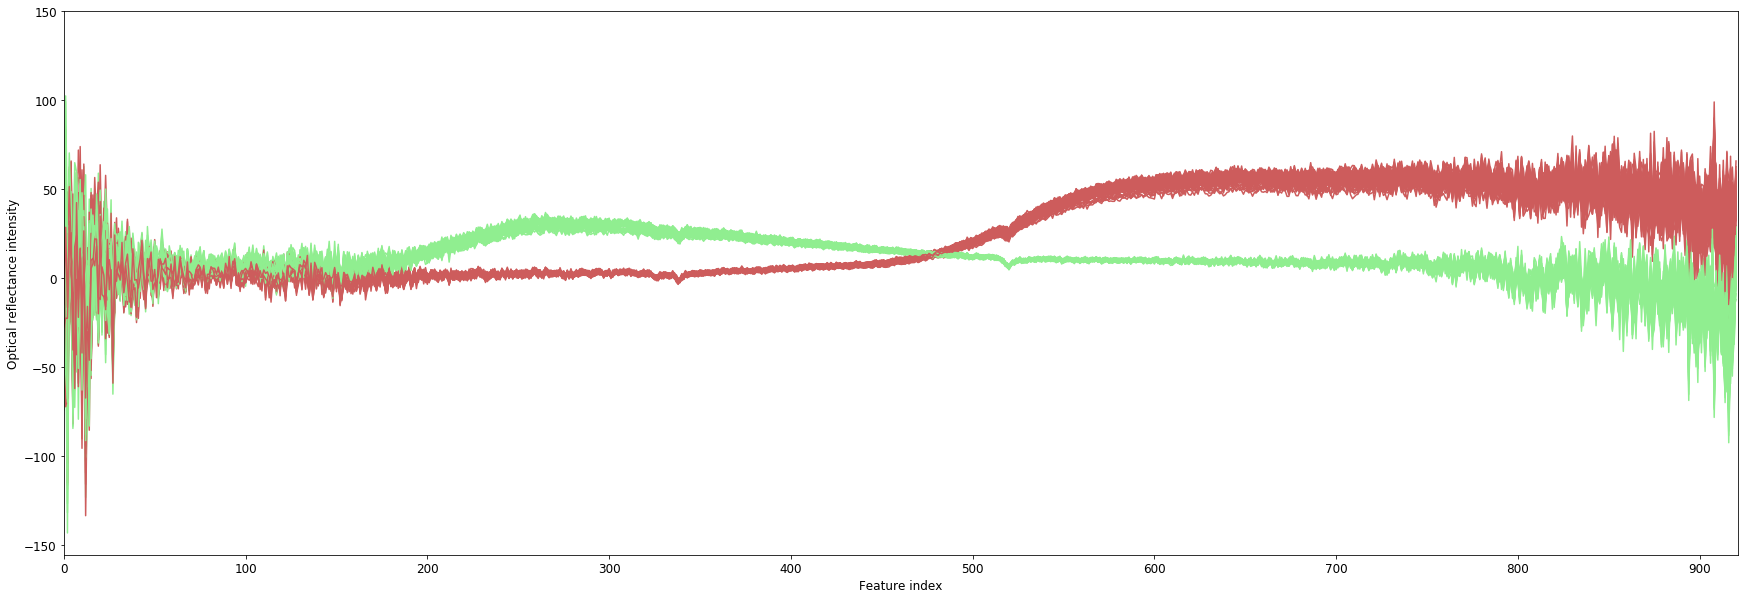
\includegraphics[width=1\textwidth]{png/binary_default}
				\caption{Input feature visualization for binary classification task. Red and green predicting samples are indicated by colour.}
				\label{fig:binary}
			\end{figure}

			Fig.\ref{fig:binary} shows that there is a clear distinction between red and green colours in terms of sample values provided in the training set. From the same figure it can be said that feature values between 0 and 100 are more or less shared between both, red and green colours. Around 470 both colour feature values overlap. Similarly, towards the final features similar observations can be made. The graph insights suggest that overlapping features are not great for determining the class because a feature value can be shared by both colours therefore reducing possibility of determining the right colour. However, a single feature that is around 300 or 650 should be good enough to determine the class. From fig.\ref{fig:binary} it is clear that intensity at those wavelengths are distinct to each colour.

			The hypothesis therefore is that any feature that distinguishes the two colours at particular wavelength will be good enough to determine the class. According to the fig.\ref{fig:binary} there are many of these features: at wavelengths in features 200-to-420 and 520-to-800. Therefore, one feature should be enough to determine the class.

		\subsection{Preparing inputs and Choosing features}

			To choose an appropriate feature an experiment was conducted. A single feature could possibly determine a class therefore a training was done using every single feature separately to determine which one is the most accurate. Fig.\ref{fig:binary_one} shows the results. Y axis represents accuracy score and X axis represents a single feature 0-to-920. 

			\begin{figure}[H]
				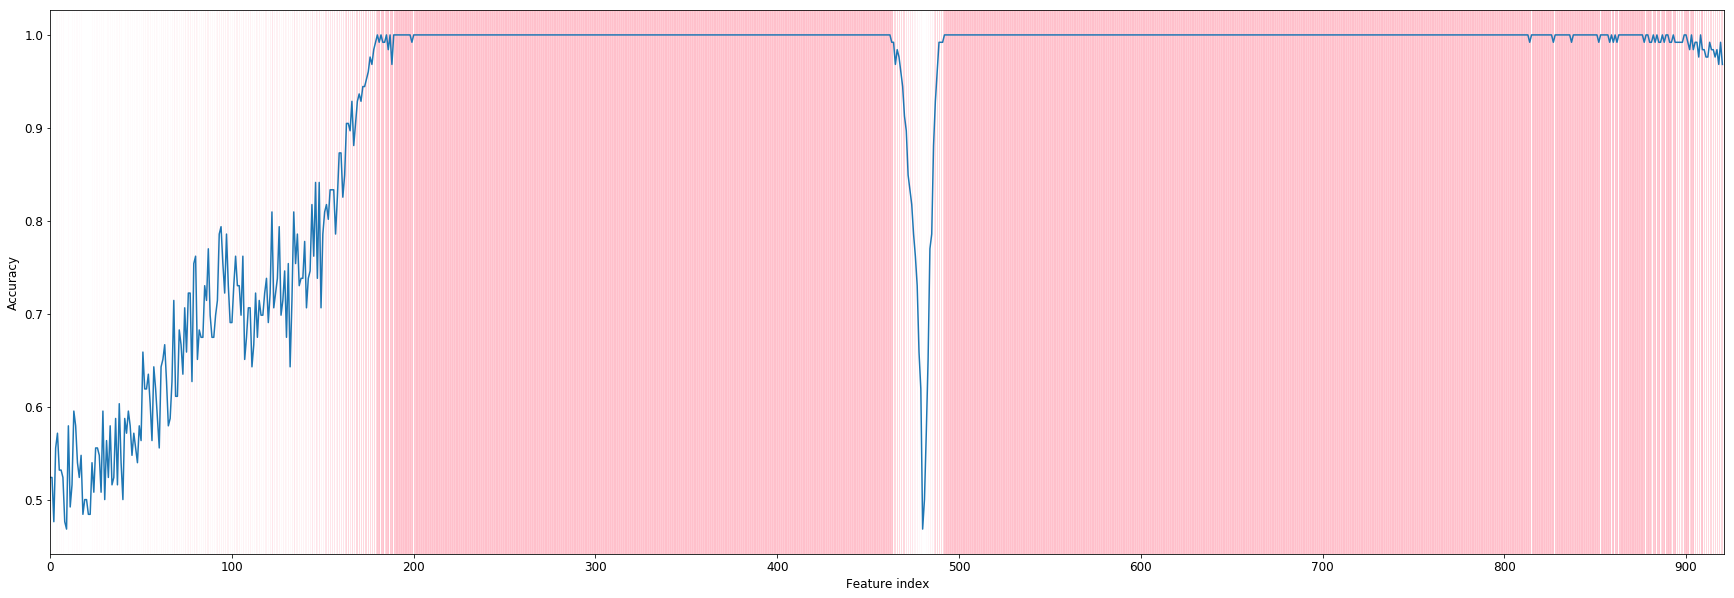
\includegraphics[width=1\textwidth]{png/binary_one}
				\caption{One feature accuracy scores for binary classification task.}
				\label{fig:binary_one}
			\end{figure}
			Pink areas cover features that perform very well. It can be seen that features indexed 200-470 and 490 to almost the end of 900 perform with 100\% accuracy. Therefore, any feature that falls in between these boundaries will perform very well. The results graph very well fits the original feature graph in fig.\ref{fig:binary} and shows that most feature values are far away for both classes apart from beginning and middle. From the graphs, large number samples also should not be necessary because there are no noticeable outliers. 

		\subsection{Selecting and Training classification model}
			\subsubsection{Linear logistic regression}
				For binary classification task a simple linear logistic regression model was chosen from sklearn. As expected, the accuracy score is 1.0 when testing with training data only. Similar observations are made by using multiple other features as shown before. This was achieved in the experiment described before. The 1.0 accuracy also means that precision and recall also 1.0 - all classes were predicted correctly. 

				Once might think that this is caused by over-fitting however from the feature analysis the results make sense. Therefore, scaling which is normally incorporated when over-fitting is suspected was not applied in this situation. 

				Since a simple linear logistic regression models seemed to work well no other models were investigated.

		\subsection{Evaluating model performance}
			\subsubsection{Linear logistic regression}
				Tbl.\ref{tbl:binary_test_table} shows results when running the model on test set using four different features. The accuracy score is 100\% in each case as expected. Form the results, it can be said that model works very well on test data when testing during four different occasions, each with different feature: 300, 400, 600 or 700 - shown in table \ref{tbl:binary_test_table}.
			
			\begin{center}
			  	\begin{table}[h]
			  	\centering
				\begin{tabular}[b]{|c | c|}
					 \hline
					 Feature Index 	 & Accuracy \\ 
	 				 \hline
					 300 				& 1.0 	\\ 
					 400 				& 1.0 	\\ 
					 600		 		& 1.0 	\\ 
					 700				& 1.0 	\\ 
					 \hline
				\end{tabular}
				\caption{Accuracy score when testing linear logistic regression model on testing set.}
				\label{tbl:binary_test_table}
				\end{table}
			\end{center}
			\vspace*{-1.5cm}

		\subsection{Result discussion}
			Results seem to be in according to the observations and hypothesis made during data investigation and visualization steps. The results suggest that both object colours can be distinguished accurately by using a single feature on certain wavelength.

			For final model for \textit{XToClassify} 400 feature was used - chosen arbitrarily. 

			\clearpage
	\section{Multi-class task}
		\subsection{Cleaning data and Feature extraction}
			Similarly to binary task, no cleaning or feature extraction was necessary. Null value function was applied on this data set too however no samples were matched. Mean, minimum and maximum values seem to be reasonable considering the features. 

		\subsection{Data analysis and Visualization}

			\begin{figure}[H]
				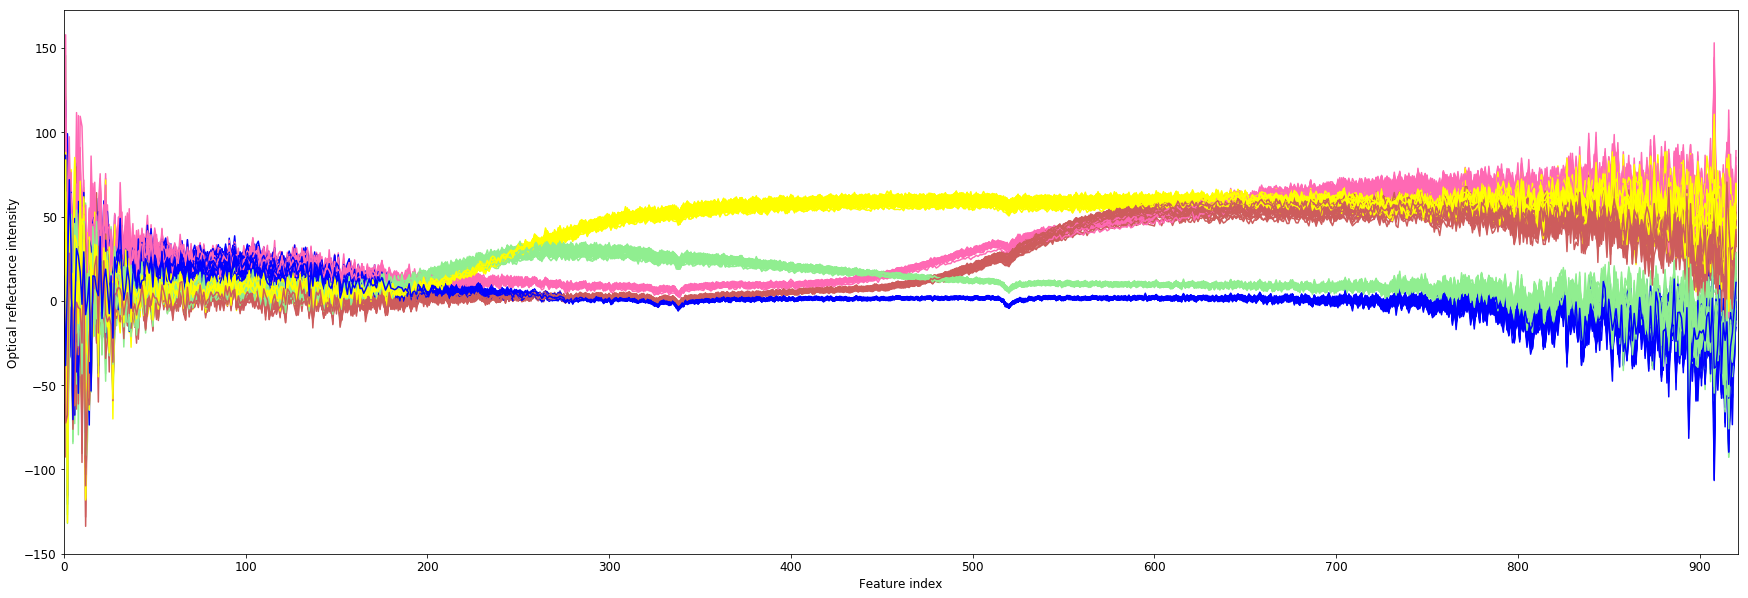
\includegraphics[width=1\textwidth]{png/multi_default}
				\caption{Input feature visualization for multi-class task. Five colour predicting samples are indicated by corresponding colour.}
				\label{fig:multi}
			\end{figure}

			Fig.\ref{fig:multi} shows different colour reflectance intensities for five different colours. Green and red just like in binary task are distinct and the same patterns can be recognized in multi-class task. However, due to larger number of colour classes some seem to overlap slightly. From fig.\ref{fig:multi} it can be seen that red and pink colour intensities over different wavelengths are very similar. Yellow on the other hand has very distinct reflectance measures. Just from looking at the graph first two hundred features do not distinct different colours. Blue and green seem to have similar reflectance towards the end. Pink, yellow and red also share similar patterns. 

			From the same graph it can also be seen that some features distinct colours well. For instance, feature indexed 420 is likely to perform well. Since there are almost no overlapping feature values for any of the colours. 

			For instance, when feature 400 is selected histogram in fig.\ref{fig:400_900} shows that the sample values are clearly distinctly distributed. Whereas feature 900 in fig.\ref{fig:400_900} shows that green and blue overlap, red pink and yellow follow the pattern. This and the original graph also suggest that blue and green will be most likely to be mixed. Pink, red and yellow mixed together too. 

		\begin{figure}
			\hfill
				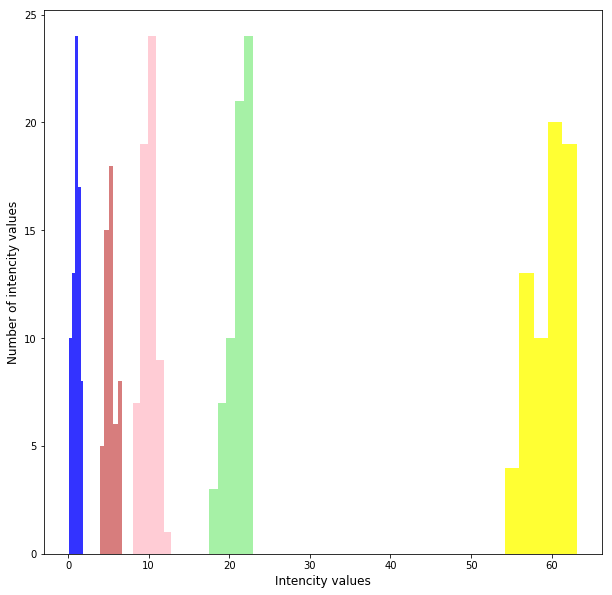
\includegraphics[width=0.4\textwidth]{png/400_multi.png}
			\hfill
				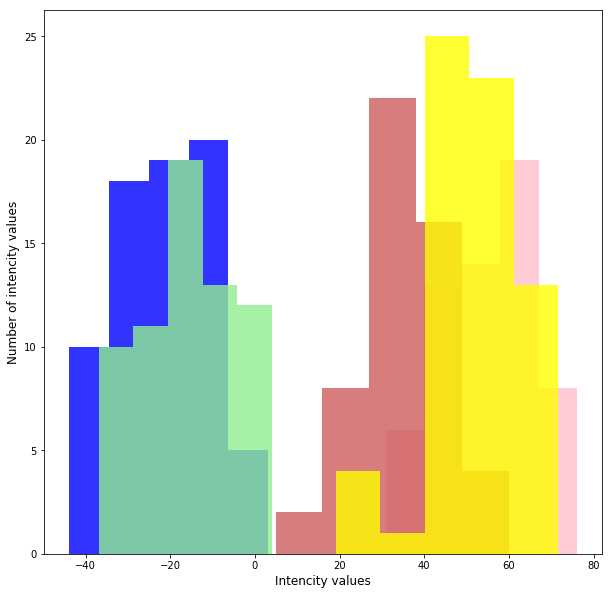
\includegraphics[width=0.4\textwidth]{png/900_multi.png}
			\hfill
			\caption{On the left - feature 400, on the right - feature 900.}
			\label{fig:400_900}
		\end{figure}

		\subsection{Preparing inputs and Choosing features}
			\begin{figure}[H]
				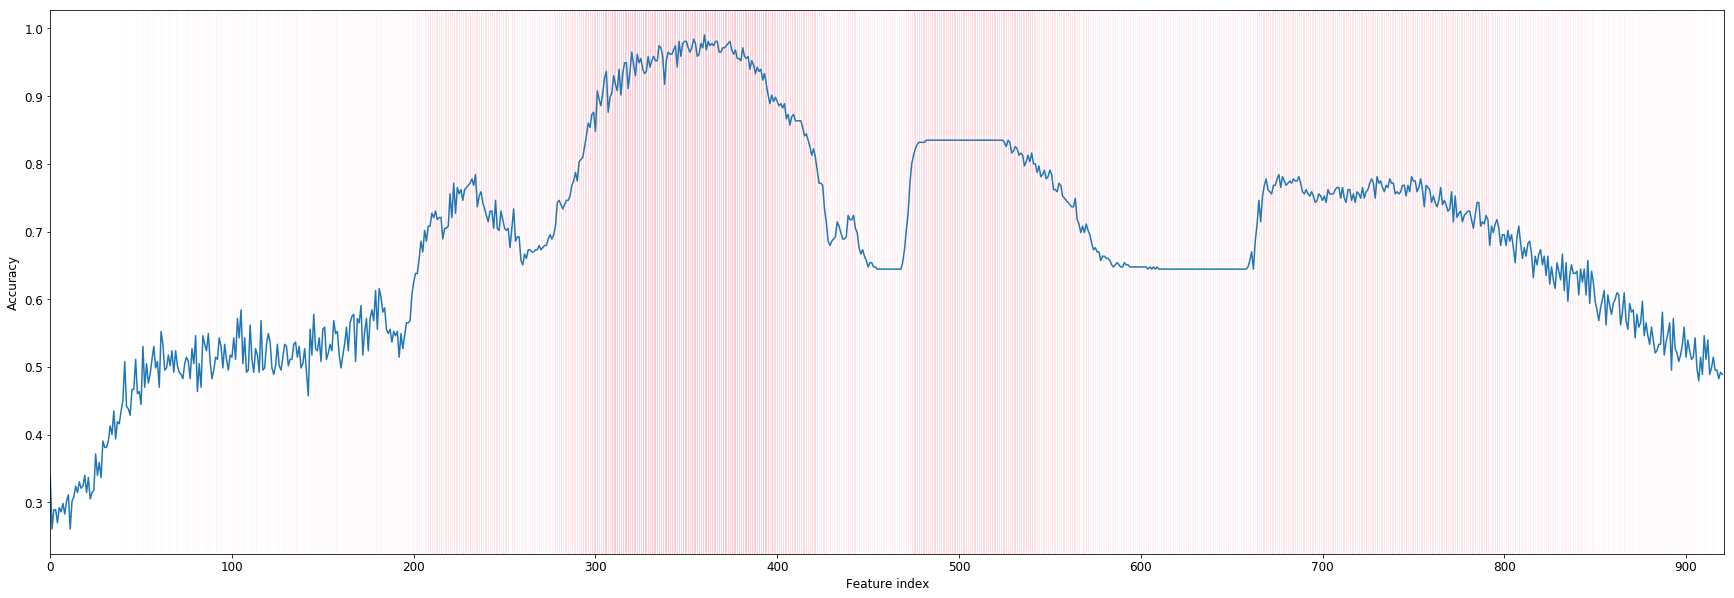
\includegraphics[width=1\textwidth]{png/multi_one}
				\caption{One feature accuracy scores for multi-class classification.}
				\label{fig:multi_one}
			\end{figure}

			Just like in binary task, in order to investigate single feature performance logistic regression model was trained on every feature separately. Fig.\ref{fig:multi_one} demonstrates the results. From the graph it can be seen that some features perform better than others. As per previous input analysis, best accuracy features are 300-to-400, providing $>$85\% accuracy on training set however not reaching 100\%. In particular, feature 350 provides over 0.9 accuracy score. Logistic regression model performance is clearly not as great as in binary task. However, still very good. To investigate further and see whether different input combinations provide better accuracy results recursive feature elimination (RFE) algorithm was used from sklearn. The idea behind this selection algorithm is to choose the best features by considering lesser number of them. Starting from the full input set the predictor recursively tries smaller subsets of inputs \cite{rfe}. The result is mask of true and false values that can be used to choose the best features. 

			For RFE experiment 1-to-10 features were chosen and accuracy scores for each selection were recorded in table \ref{tbl:accuracy_table} below.

		\begin{center}
		  	\begin{table}[h]
		  	\centering
			\begin{tabular}[b]{|c | l | c|}
				 \hline
				 No & Feature indexes 	  						    & Accuracy \\ 
				 \hline
				 1 & 421 											& 0.810 \\ 
				 2 & 421, 429 										& 0.851 \\ 
				 3 & 421, 429, 250 									& 0.997 \\ 
				 4 & 421, 429, 250, 251 							& 0.997 \\ 
				 5 & 421, 429, 250, 251, 86 						& 1.0 	\\ 
				 6 & 421, 429, 250, 251, 86, 586 					& 1.0 	\\ 
				 7 & 421, 429, 250, 251, 86, 586, 88 				& 1.0 	\\ 
				 8 & 421, 429, 250, 251, 86, 586, 88, 66 			& 1.0 	\\ 
				 9 & 421, 429, 250, 251, 86, 584, 88, 66, 586 		& 1.0 	\\ 
				 10 & 421, 429, 250, 251, 86, 584, 88, 66, 586, 914 & 1.0 	\\ 
				 \hline
			\end{tabular}
			\caption{Accuracy table for different features. }
			\label{tbl:accuracy_table}
			\end{table}
		\end{center}
		\vspace*{-1.3cm}

		This table shows how many features is the optimal number for maintaining good accuracy score. With feature 421 accuracy score is 0.81 which is already very good. As the number of features is increased the accuracy score also becomes higher. Three features - 421, 429 and 250 are enough to achieve almost 1.0 accuracy. Later, as the number of features is more than four the accuracy score is stable and is 1.0.

		Interestingly, the RFE did not choose 350 feature although as the previous experiment suggests it provides over 0.9 accuracy score on its own. This might be because RFE chooses features by eliminating a subset of features - large subset of features means better accuracy however elimination does not diverge to a single optimal feature. 

		After analysis, a subset of three features was chosen: 421, 429 and 250. This subset resulted in 0.997 accuracy on training set when experimenting.

		\subsection{Selecting and Training classification models}
			\subsubsection{Linear logistic regression model}
 			 	When using linear regression model with the three features accuracy of 0.997 is achieved on training set. Table \ref{tbl:logistic_resuts_multi} holds classification report results. Each class has a precision, recall, f1-score and support measures. 

 			 	It can be seen that only green and pink have precision or recall other than 1.0. Precision indicates what part of positive classifications were actually correct whereas recall what part of actual positives were identified correctly. F-1 score is a weighted average of both precision and recall. Support identifies the number of actual classifications for particular class.

 			 	From the totals it can be said that the linear logistic regression model seems to be a very good model for this particular problem. 

			\begin{center}
			  	\begin{table}[h]
			  	\centering
				\begin{tabular}[b]{| l | c | c | c | c | c |}
					\hline
					Class & Class No & Precision &  Recall & F1-score & Support  \\
		 			\hline
					  Blue  &  0  &    1.00   &   1.00   &   1.00    &    72 \\
			          Green &  1  &    0.98   &   1.00   &   0.99    &    65 \\
			          Pink  &  2   &    1.00   &   0.98   &   0.99    &    60 \\
			          Red  &   3   &    1.00   &   1.00   &   1.00    &    52 \\
			          Yellow & 4   &    1.00   &   1.00   &   1.00    &    66 \\
		  			\hline
					 & avg / total   &    1.00   &   1.00   &   1.00   &    315 \\
					\hline
				\end{tabular}
				\caption{Logistic regression report results on training data.}
				\label{tbl:logistic_resuts_multi}
				\end{table}
			\end{center}
			\vspace*{-1.3cm}
			\subsubsection{Linear vector support classifier}
				To experiment further, a linear vector support classifier was applied on the same three features. Accuracy of 1.0 was achieved. This is slightly better than the logistic regression model results. 

				From the table \ref{tbl:vector_resuts_multi} it can be observed that the averages are just like in logistic regression model. However, vector support model seems to perform better with colours pink and green achieving 1.0 in precision and recall. 
			
			\begin{center}
			  	\begin{table}[h]
			  	\centering
				\begin{tabular}[b]{| l | c | c | c | c | c |}
					\hline
					Class & Class No & Precision &  Recall & F1-score & Support  \\
		 			\hline
					Blue & 0  &   1.00   &   1.00   &   1.00   &   72 \\
          			Green & 1  &   1.00   &   1.00   &   1.00   &    65 \\
         			Pink & 2  &   1.00   &   1.00   &   1.00   &     60 \\
          			Red & 3  &   1.00   &   1.00   &   1.00   &     52 \\
          			Yellow & 4  &   1.00   &   1.00   &   1.00   &     66 \\
          			\hline
					 & avg / total   &   1.00   &   1.00   &   1.00  &      315 \\
					\hline
				\end{tabular}
				\caption{Linear support vector classifier report results on training data.}
				\label{tbl:vector_resuts_multi}
				\end{table}
			\end{center}
			\vspace*{-1.3cm}

 			 The results table tells that there are more blue colour samples in the training set than any other colour. Red has the smallest number of samples. This would normally indicate that the model could possibly perform better when classifying certain classes however in this case this does not apply.

		\subsection{Evaluating model performance on testing set}

			From the two models chosen support vector classifier performs slightly better therefore is chosen for testing on test data set. The three same input features are used.

			The results of the model performance are recorded in table \ref{tbl:vector_resuts_multi_testing}. The same observations can be made as with training data. The chosen futures and the VSC seems to provide 1.0 accuracy. The results tell that all of the test samples were classified correctly. Due to used cross validation and input observations this is not likely to be caused by over-fitting. The data provided seems to be excellent for classifying especially when extracting the right features which was achieved successfully using the RFE approach.  

			\begin{center}
			  	\begin{table}[h]
			  	\centering
				\begin{tabular}[b]{| l | c | c | c | c | c |}
					\hline
					Class & Class No & Precision &  Recall & F1-score & Support  \\
		 			\hline
					Blue  & 0  &   1.00   &   1.00   &   1.00   &   18 \\
          			Green & 1  &   1.00   &   1.00   &   1.00   &   25 \\
         			Pink  & 2  &   1.00   &   1.00   &   1.00   &   30 \\
          			Red  & 3  &   1.00   &   1.00   &   1.00   &   38 \\
          			Yellow & 4  &   1.00   &   1.00   &   1.00   &  24 \\
          			\hline
					 & avg / total   &   1.00   &   1.00   &   1.00  &  135 \\
					\hline
				\end{tabular}
				\caption{Linear support vector classifier report results on test data.}
				\label{tbl:vector_resuts_multi_testing}
				\end{table}
			\end{center}
			\vspace*{-1.3cm}

		\subsection{Result discussion}
			I first considered applying scaling techniques but the final models performed very well on the test data too. Therefore, this step was skipped. Also, data is already to some extend scaled the values are in range from -150 to 150. However, I do understand that it is good practice in general to apply scaling and normalization techniques. I believe in this case it is not necessary. 

			From the results both logistic regression and VSC are good for the multi-class classification task. 

	\section{Conclusion}
		This practical submission contains two python notebooks: one for each task. As per practical specification, appendices section of this report contains two tables for each of the task final predictions for \textit{XToClassify}. Directories \textit{/binaryTask/} and \textit{/multiClassTask/} contain files with the same results. 

		Data was clean and ready for machine learning. Overall, this submission investigated data sets through different visualization techniques, then it applied multiple machine learning models and observed and reported results using common classification measures in results tables. From binary and multi-class classification results both models perform very well. Due to previously stated facts this is unlikely to be due to over-fitting. 

		Because of good results I did not explore more models. The two simple logistic and VSC models were well-suited for these two tasks. 

		From the data observations the models should perform well on a very small training sample too e.g, five samples - one for each of the class for multi-class task and two for binary classification. If had more time, this I believe could be proved too. 

	\clearpage
	\appendix
	\section{Appendices}
		\subsection{Binary task results}
		\begin{center}
		  	\begin{table}[h]
		  		\small

		  	\centering
	  	 	% \resizebox{0.2\textwidth}{!}{%

			\begin{tabular}[b]{| c | c|} 
				\hline
				No & Class \\
				\hline
				1 & 1 \\ 2 & 1 \\ 3 & 0 \\ 4 & 0 \\ 5 & 1 \\ 6 & 0 \\ 7 & 0 \\ 8 & 0 \\ 9 & 1 \\ 10 & 0 \\
				\hline
			\end{tabular}
			% }
			\begin{tabular}[b]{| c | c|} 
				\hline
				No & Class \\
				\hline
				11 & 0 \\ 12 & 1 \\ 13 & 1 \\ 14 & 1 \\ 15 & 0 \\ 16 & 1 \\ 17 & 1 \\ 18 & 0 \\ 19 & 1 \\ 20 & 0 \\
				\hline
			\end{tabular}
			\caption{Binary task result for \textit{XToClassify}.}
			\label{tbl:final_binary}
			\end{table}
		\end{center}


		\subsection{Multi-class task results}


		\begin{center}
		  	\begin{table}[h]
		  		\small

		  	\centering
			\begin{tabular}[b]{| c | c|} 
				\hline
				No & Class \\
				\hline
				1 & 2 \\ 2 & 0 \\ 3 & 2 \\ 4 & 0 \\ 5 & 0 \\ 6 & 0 \\ 7 & 2 \\ 8 & 0 \\ 9 & 4 \\ 10 & 1\\ 
				\hline
			\end{tabular}
			\begin{tabular}[b]{| c | c|} 
				\hline
				No & Class \\
				\hline
				 11 & 4 \\ 12 & 3 \\ 13 &  3 \\ 14 &  2\\ 15 &  0\\ 16 & 4\\ 17 & 2\\ 18 &  4 \\ 19 &  3\\20 & 3 \\ 
				\hline
			\end{tabular}
			\begin{tabular}[b]{| c | c|} 
				\hline
				No & Class \\
				\hline
				 21 & 4 \\ 22 &  1 \\ 23 & 2 \\ 24 & 1 \\ 25 & 4 \\ 26 & 2 \\ 27 & 3 \\ 28 & 2 \\ 29 & 0 \\ 30 & 1 \\ 
				\hline
			\end{tabular}
			\begin{tabular}[b]{| c | c|} 
				\hline
				No & Class \\
				\hline
				 31 & 1 \\ 32 & 1 \\ 33 & 3 \\ 34 & 1 \\ 35 & 2 \\ 36 & 4 \\ 37 & 2 \\ 38 & 3 \\ 39 & 1 \\ 40 & 4 \\
				\hline
			\end{tabular}
			\begin{tabular}[b]{| c | c|} 
				\hline
				No & Class \\
				\hline
				 41 & 0 \\ 42 & 0 \\ 43 & 1 \\ 44 & 1 \\ 45 & 3 \\ 46 & 0 \\ 47 & 3 \\ 48 & 4 \\ 49 & 3 \\ 50 & 4 \\
				\hline
			\end{tabular}
			\caption{Binary task result for \textit{XToClassify}.}
			\label{tbl:final_binary}
			\end{table}
		\end{center}
	\clearpage

	\begin{thebibliography}{9}

		\bibitem{rfe} 
		Sklearn RFE [Accessed 21/04/2018]
		\\\texttt{http://scikit-learn.org/stable/modules/generated/sklearn.feature\_selection.RFE.html}

	\end{thebibliography}
\end{document}  